% Generated by pysimcount.pfseeds -- do not edit; regenerate instead.
% figure: B-all-by-formula -- Every formula at measured r; median over seeds [1, 2, 3, 4, 5], bars = min..max
% metric=total gatebase=cz merged
% seed 1: git_commit=04cd66abb614bdc66fb48e891cef085a299e0ab1 git_dirty=False
% seed 2: git_commit=04cd66abb614bdc66fb48e891cef085a299e0ab1 git_dirty=False
% seed 3: git_commit=04cd66abb614bdc66fb48e891cef085a299e0ab1 git_dirty=False
% seed 4: git_commit=04cd66abb614bdc66fb48e891cef085a299e0ab1 git_dirty=False
% seed 5: git_commit=04cd66abb614bdc66fb48e891cef085a299e0ab1 git_dirty=False
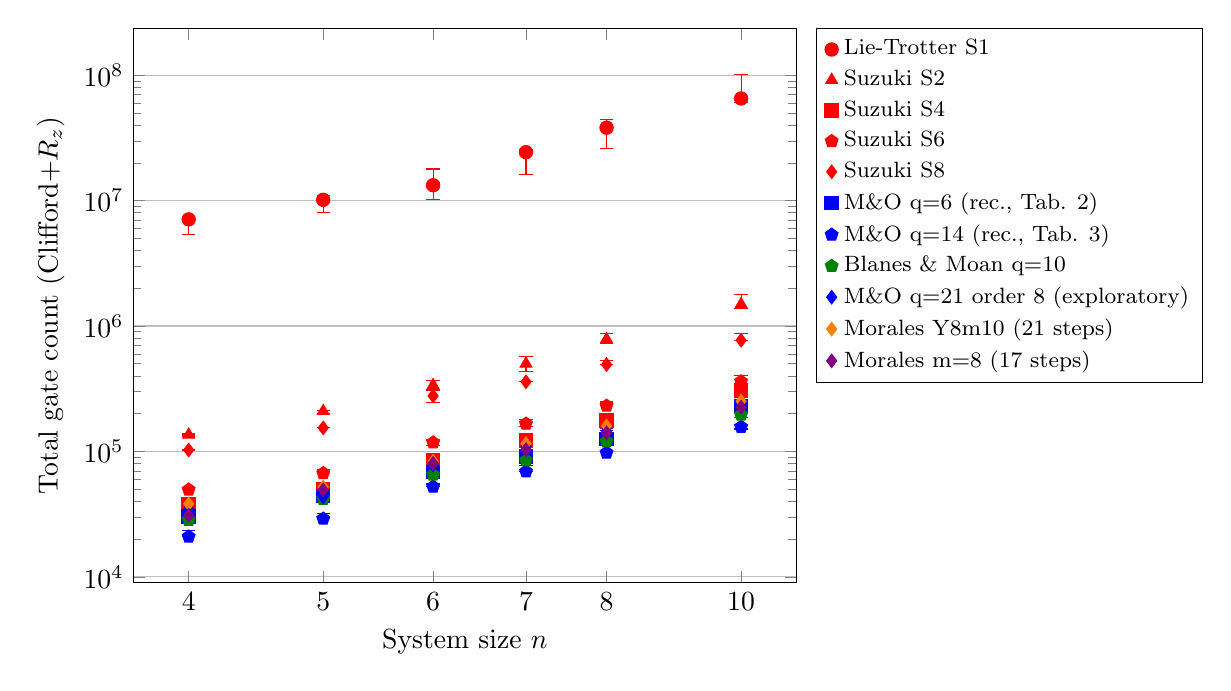
\begin{tikzpicture}
  \begin{loglogaxis}[
    width=10cm,
    xlabel={System size $n$},
    ylabel={Total gate count (Clifford+$R_z$)},
    xtick={4,5,6,7,8,10},
    xticklabels={4,5,6,7,8,10},
    ymajorgrids=true,
    legend pos=outer north east,
    legend cell align=left,
    legend style={font=\footnotesize},
  ]
    \addplot[only marks, red, mark=*, mark size=2.4pt, mark options={solid, fill=red}, error bars/.cd, y dir=both, y explicit, error bar style={red}] coordinates {
      (4,7085000) += (0,255112) -= (0,1725672)
      (5,10143770) += (0,837720) -= (0,2101450)
      (6,13264524) += (0,4627272) -= (0,3001596)
      (7,24325028) += (0,1252888) -= (0,8051134)
      (8,38159472) += (0,5941936) -= (0,12316720)
      (10,65251680) += (0,36193040) -= (0,4422340)
    };
    \addlegendentry{Lie-Trotter S1}
    \addplot[only marks, red, mark=triangle*, mark size=2.4pt, mark options={solid, fill=red}, error bars/.cd, y dir=both, y explicit, error bar style={red}] coordinates {
      (4,135936) += (0,1728) -= (0,3264)
      (5,209520) += (0,1920) -= (0,7440)
      (6,337248) += (0,31968) -= (0,25920)
      (7,500640) += (0,70896) -= (0,65184)
      (8,785664) += (0,91008) -= (0,59136)
      (10,1489440) += (0,294720) -= (0,107040)
    };
    \addlegendentry{Suzuki S2}
    \addplot[only marks, red, mark=square*, mark size=2.4pt, mark options={solid, fill=red}, error bars/.cd, y dir=both, y explicit, error bar style={red}] coordinates {
      (4,38160) += (0,848) -= (0,848)
      (5,49820) += (0,6360) -= (0,2120)
      (6,85224) += (0,5088) -= (0,5088)
      (7,121688) += (0,17808) -= (0,7420)
      (8,176384) += (0,11872) -= (0,5088)
      (10,305280) += (0,33920) -= (0,8480)
    };
    \addlegendentry{Suzuki S4}
    \addplot[only marks, red, mark=pentagon*, mark size=2.4pt, mark options={solid, fill=red}, error bars/.cd, y dir=both, y explicit, error bar style={red}] coordinates {
      (4,49536) += (0,0) -= (0,0)
      (5,67080) += (0,5160) -= (0,0)
      (6,117648) += (0,6192) -= (0,6192)
      (7,166152) += (0,14448) -= (0,7224)
      (8,231168) += (0,16512) -= (0,0)
      (10,361200) += (0,41280) -= (0,10320)
    };
    \addlegendentry{Suzuki S6}
    \addplot[only marks, red, mark=diamond*, mark size=2.4pt, mark options={solid, fill=red}, error bars/.cd, y dir=both, y explicit, error bar style={red}] coordinates {
      (4,102640) += (0,0) -= (0,0)
      (5,153960) += (0,0) -= (0,0)
      (6,277128) += (0,30792) -= (0,30792)
      (7,359240) += (0,0) -= (0,0)
      (8,492672) += (0,41056) -= (0,0)
      (10,769800) += (0,102640) -= (0,0)
    };
    \addlegendentry{Suzuki S8}
    \addplot[only marks, blue, mark=square*, mark size=2.4pt, mark options={solid, fill=blue}, error bars/.cd, y dir=both, y explicit, error bar style={blue}] coordinates {
      (4,30360) += (0,0) -= (0,1012)
      (5,44275) += (0,0) -= (0,0)
      (6,68310) += (0,0) -= (0,3036)
      (7,90321) += (0,5313) -= (0,5313)
      (8,125488) += (0,8096) -= (0,8096)
      (10,225170) += (0,2530) -= (0,10120)
    };
    \addlegendentry{M\&O q=6 (rec., Tab. 2)}
    \addplot[only marks, blue, mark=pentagon*, mark size=2.4pt, mark options={solid, fill=blue}, error bars/.cd, y dir=both, y explicit, error bar style={blue}] coordinates {
      (4,20916) += (0,2324) -= (0,0)
      (5,29050) += (0,2905) -= (0,0)
      (6,52290) += (0,3486) -= (0,0)
      (7,69139) += (0,8134) -= (0,0)
      (8,97608) += (0,4648) -= (0,0)
      (10,156870) += (0,5810) -= (0,5810)
    };
    \addlegendentry{M\&O q=14 (rec., Tab. 3)}
    \addplot[only marks, green!50!black, mark=pentagon*, mark size=2.4pt, mark options={solid, fill=green!50!black}, error bars/.cd, y dir=both, y explicit, error bar style={green!50!black}] coordinates {
      (4,28356) += (0,1668) -= (0,0)
      (5,41700) += (0,0) -= (0,0)
      (6,65052) += (0,0) -= (0,2502)
      (7,84651) += (0,2919) -= (0,0)
      (8,120096) += (0,0) -= (0,6672)
      (10,195990) += (0,8340) -= (0,8340)
    };
    \addlegendentry{Blanes \& Moan q=10}
    \addplot[only marks, blue, mark=diamond*, mark size=2.4pt, mark options={solid, fill=blue}, error bars/.cd, y dir=both, y explicit, error bar style={blue}] coordinates {
      (4,34720) += (0,0) -= (0,0)
      (5,43400) += (0,4340) -= (0,0)
      (6,78120) += (0,5208) -= (0,0)
      (7,109368) += (0,6076) -= (0,6076)
      (8,145824) += (0,6944) -= (0,0)
      (10,234360) += (0,26040) -= (0,8680)
    };
    \addlegendentry{M\&O q=21 order 8 (exploratory)}
    \addplot[only marks, orange, mark=diamond*, mark size=2.4pt, mark options={solid, fill=orange}, error bars/.cd, y dir=both, y explicit, error bar style={orange}] coordinates {
      (4,38192) += (0,3472) -= (0,0)
      (5,52080) += (0,4340) -= (0,0)
      (6,83328) += (0,5208) -= (0,0)
      (7,115444) += (0,6076) -= (0,6076)
      (8,159712) += (0,6944) -= (0,6944)
      (10,251720) += (0,34720) -= (0,0)
    };
    \addlegendentry{Morales Y8m10 (21 steps)}
    \addplot[only marks, violet, mark=diamond*, mark size=2.4pt, mark options={solid, fill=violet}, error bars/.cd, y dir=both, y explicit, error bar style={violet}] coordinates {
      (4,30976) += (0,0) -= (0,2816)
      (5,49280) += (0,3520) -= (0,0)
      (6,80256) += (0,0) -= (0,4224)
      (7,103488) += (0,4928) -= (0,0)
      (8,140800) += (0,11264) -= (0,0)
      (10,225280) += (0,14080) -= (0,7040)
    };
    \addlegendentry{Morales m=8 (17 steps)}
  \end{loglogaxis}
\end{tikzpicture}
